\documentclass[parskip=full]{aaltoseries}
\usepackage{graphicx}
\usepackage{hyperref}
\usepackage{titlesec}
\graphicspath{{images/}}
\usepackage{amsmath}
\usepackage{enumitem}
\providecommand{\inlinecode}[1]{\texttt{#1}}
\providecommand{\abs}[1]{\lvert#1\rvert}
\titleformat{\chapter}{\Large\bfseries}{\thechapter}{0pt}{\vskip 0pt\raggedright}%
\let\cleardoublepage\clearpage
\begin{document}

\title{IR Search Ranking Methods}

\tableofcontents


\chapter{Introduction}
With growing digitalization and worldwide spreading of the internet, unprecedented amounts of data is being created by users, generated automatically, processed and stored online. Researches stated as early as 2010 that every two days humanity created the same amount of information as was created since the dawn of civilization until 2003. In such circumstances it gets more and more challenging to search for information efficiently and to find relevant items.

A good ranking method is the key ingredient in optimizing search results so that they are useful to the user, and also presented in an order of ranked relevance. Search engines can use different ranking functions, text-processing techniques and overall configurations to provide the best results.

The objective of the present course project work is to get familiar with the evaluation of information retrieval by calculating the precision and recall of queries and comparing different techniques used in the search methods.

\chapter{Description of Techniques}
Two different similarity ranking methods have been chosen, Vector Space Model (VSM) and Okapi BM25. For morphological analysis, the effect of using a Porter stemmer is observed by using two different text analyzers available in Lucene: Standard Analyzer (does not provide stemming) and English Analyzer (provides stemming according to Porter Stemmer). Furthermore, the effect of filtering stopwords is observed.
\section{Similarity}
Semantic similarity is a metric for a set of documents or terms, where terms are compared on their meaning likeness. The metric is used to determine the semantic relationship between terms with the use of scoring. Similarity ranking functions, in turn, are methods used by search engines to determine appropriate scores for documents in comparison to the query. They are used to figure out whether a document is relevant at all, and if so, the magnitude of the relevancy. To correlate words and their textual contexts, different statistical means can be used. The methods used in this task are presented below.
\subsection{Vector Space Model}
In Vector Space Models documents are represented as vectors in a t-dimensional space, where t is a term. There are different ways to compute the vectors. Lucene uses a popular method, term frequency-inverse document frequency (tf-idf), to calculate the weight of the vectors. The relevancy of a document is determined by comparing the angle of the document vectors with the query vector. As of Lucene 6.0.0, the implementation of the abstract VSM class \inlinecode{TFIDFSimilarity} is the \inlinecode{ClassicSimilarity} class. It uses Vector Space Model similarity with tf-idf weighting and some adjustments for more efficient computations.
\newpage
\subsection{Okapi BM25}
Okapi BM25 is a ranking function based on probabilistic retrieval framework. Several modifications of BM25 exist, but the most common scoring function uses the following equation:
\begin{align*}
score(D,Q) &= \sum_{\substack{i=1}} IDF(q_i)*\frac{f(q_i,D)*(k_1+1)}{f(q_i,D)+k_1*(1-b+b*\frac{\abs{D}}{avgdl})} \\
\end{align*} 
Where $D$ = document, $avgdl$ = avg. doc length, $k_1$ is the parameter controlling non-linear term frequency normalization (or saturation), $b$ is the parameter controlling to what degree document length normalizes tf values, and $Q$ is the query. By default, Lucene's \inlinecode{BM25Similarity()} constructor uses the values of $k_1=1.2$ and $b=0.75$. 

Even though both algorithms use IDF, a notable difference between VSM and BM25 is that the score output in BM25 is much higher, so one should not compare the scores directly.
\section{Stopwords}
Stopwords are words that are so common and insignificant that we might wish to omit them from a search, e.g. all articles, prepositions and conjunctions. Lucene provides a \inlinecode{StopWordFilter} which filters stopwords from a document. The \inlinecode{StopWordFilter} has 33 words (presented below) but it's possible to introduce a new words to the set.

\inlinecode{[but, be, with, such, then, for, no, will, not, are, and, their, if, this, on, into, a, or, there, in, that, they, was, is, it, an, the, as, at, these, by, to, of]}

Lucene's \inlinecode{StandardAnalyzer} uses English stopwords by default. However, if language-based stopword filtering is required, Lucene has \inlinecode{Analyzer} packages for almost all languages available. Those packages contain localized stopwords sets.


\newpage
\section{Stemming}
Stemming is the act of normalizing words into their simplest form. E.g. conjugated and plural words are shortened down to their root verb and singular versions. The benefit of stemming is matching a query term with a very similar word, which in context may have the exact same meaning. One such stemming algorithm is called Porter stemmer. It takes words as inputs and replaces substrings with shorter substrings, single characters, or whitespace. Not all words can be stemmed, as they may already be at their root, e.g. 'argument' is already stemmed, whereas 'arguments' will have its pluralized 's' removed. When stemming documents, the query must be stemmed as well. As an example, the stemmed search query can be found below:

\inlinecode{cross-language information retrieval:} \newline
\inlinecode{(abstract\_text:cross abstract\_text:languag)
\newline abstract\_text:inform abstract\_text:retriev}

The \inlinecode{EnglishAnalyzer} in Lucene is an analyzer class which includes some useful filters for normalizing a document, among them a lowercase filter, a stopword filter, and a Porter stemmer.

\chapter{Evaluation of Techniques}
We implemented a Java application that uses Lucene and the abovementioned search configurations, giving us a total of six different combinations:
\begin{itemize}[noitemsep]
\item Vector Space Model with English Analyzer and stopwords
\item Vector Space Model with English Analyzer and no stopwords
\item Vector Space Model with Standard Analyzer and stopwords
\item BM25 with English Analyzer and stopwords
\item BM25 with English Analyzer and no stopwords
\item BM25 with Standard Analyzer and stopwords
\end{itemize}
There were three similar queries we were searching with on the topic of "cross-language information retrieval", leaving us with a total of 18 different precision-recall sets. To produce an 11-step interpolated precision-recall curve, the values of precision and recall were averaged for all searches in each of the configurations. Then, the closest recall values and the corresponding interpolated precision values were found for 0.0 - 1.0 interval with a step of 0.1. 

For VSM cosine similarity with tf-idf we were using \inlinecode{ClassicSimilarity()} class that extends \inlinecode{TFIDFSimilarity()}. For stemming, \inlinecode{EnglishAnalyzer()} was used with an additional parameter \inlinecode{CharArraySet.EMPTY\_SET} no exclude stopwords. For no stemming, \inlinecode{StandardAnalyzer()} was sufficient. As standard analyzer class was still using English stopwords by default, optional parameter \inlinecode{CharArraySet.EMPTY\_SET} was required to exclude stopwords. For BM25 similarity BM25Similarity() class was used. For stemming and stopwords settings  same techniques were used as for the \newline \inlinecode{ClassicSimilarity()}. Configuration specification was required for both indexing the documents with \inlinecode{IndexWriter()} and searching through the document collection with \inlinecode{IndexSearcher()}. For the search query, \inlinecode{QueryParser()} class was used, that allowed us to parse a string to match Lucene query syntax. Also, \inlinecode{QueryParser()} was considering Analyzer settings to decide e.g. whether to stem the query/remove stopwords or not. 
After searching through the document collection the results were scored and stored in the \inlinecode{ScoreDoc[]} type array. By checking if the document returned was really relevant or false-relevant, precision and recall rates were computed. We were using the following formulas for precision and recall: 
\begin{align*}
Precision = \frac{RelevantItemsRetrieved}{RetrievedItems}
\end{align*} 
\begin{align*}
Recall = \frac{RelevantItemsRetrieved}{RelevantItems}
\end{align*} 
After getting precision and recall for each of the documents returned from search, precision values were interpolated for each tenth fraction of recall. 

\begin{figure}[!ht]
\caption{11-step interpolated precision recall curve}
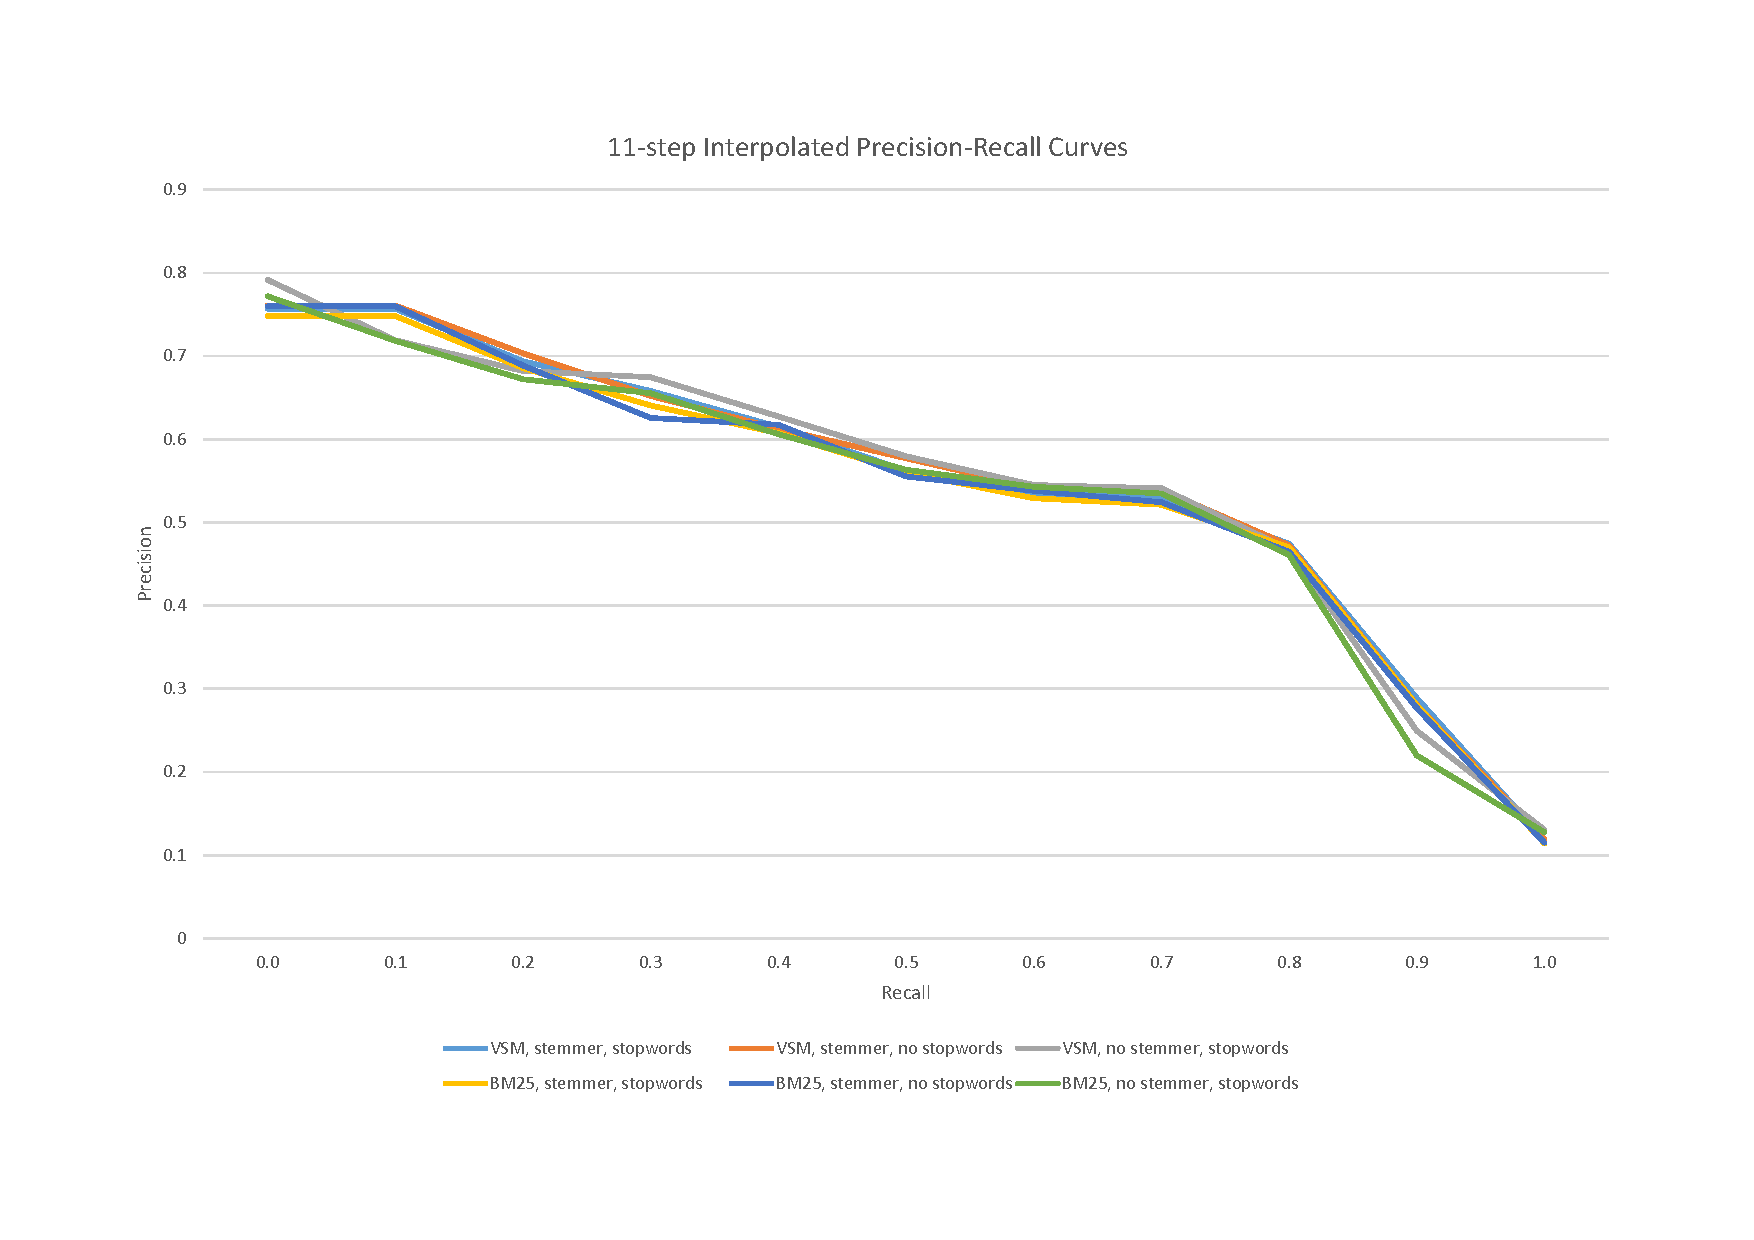
\includegraphics[scale=0.40]{curves.pdf}
\end{figure}

While implementing the search methods we discovered a number of interesting search behaviours. First of all, the overall precision and recall rates didn't change much for VSM with different configuration as well as for BM25. However, when looking at precision rates for the specific recall points, the differences existed. Obviously, precision was changing because of the document order changes in returned search results. 
Secondly, we had to search through the whole document collection and not just the documents assigned to our group to get a more clear view on the differences between the search models. We made this decision because it turned out that the precision rate was more than 80\% almost for all search case scenarios. 
Thirdly, it turned out that the usage of the Porter stemmer and stopwords set do not produce much of a difference for the final set of results.  
\chapter{Conclusions}
While there is a noticeable difference between average interpolated precision levels of different search configurations, this difference is not very significant. We revised and re-wrote the code many times, but we were not able to achieve any other result than presented in this report. Based on the results, we come to following conclusions:
\begin{itemize}
\item There is very small difference between Vector Space Model and Okapi BM25 ranking functions.
\item Including and excluding words from the default stopword list does not affect search engine performance.
\item Disabling stemming provides slightly worse precision values, as can be observed at recall levels 0.1 and 0.9.
\end{itemize}
We also identified a number of concerns that we were unable to resolve in course of this project work:
\begin{itemize}
\item We are not sure if we are using Lucene correctly, as the documentation is hard to explore, sometimes difficult to understand and clearly aimed at professionals. We did not find much help online, as most online references were made considering outdated versions of Lucene.
\item We are not sure if our set of search queries suits the task well. We were unable to observe significant differences while using other search queries.
\end{itemize}
Nevertheless, we believe that our objectives for this project are complete, as we were able to use Lucene search engine library to create a text corpus, to search this corpus with given queries and to obtain relevant results, using relatively simple techniques for search engine configuration. We observed a slight difference in ranking functions performance and used 11-step interpolated precision-recall curves to plot this difference.

\chapter{Work Distribution}
Our team has worked closely during all the stages of this project. We had weekly meetings to discuss the current process and decide on the next steps. During the first meeting we decided to use git version control software to conveniently monitor all the changes in the code. We also decided to have a number of programming sessions, where we could brainstorm the solutions to the issues and discuss the best techniques to use. Google Docs was chosen for writing all the documentation, because it allowed to see all the changes in real-time. Facebook chat functionality was chosen as a main communication method because of its simplicity and availability for all the team members.

We believe that the initial arrangements worked out well. First, Rodion and Mathias made a research on VSM with tf-idf and BM25 ranking methods and their application in Lucene, while Anton refactored the code from assignment 1 to work for the new document collection and search queries. After that, we added ranking and different settings for the analyzers during the programming session. 
As no sample outputs were provided in the assignment, we had to make a lot of assumptions on the accuracy of the results, which is why we spent plenty of time trying to find errors and understand if the program was behaving in the right way. At some point the code started to look too complicated and the decision was made to divide into teams: Anton and Mathias were adding functionality and debugging the current code, while Rodion was using it to rewrite the program from scratch applying object-oriented approach. As a result, at some point we started to use the new java classes and the old code got retired. \newline During the last programming session we added the functionality that was required to produce 11-step interpolated precision recall curve. It was not as trivial as we initially supposed, so some code had to be re-written. While Anton and Rodion were trying to overcome new problems, Mathias researched the Latex document format and started to prepare everything for the report creation. \newline In the end, all team members took part in writing this report. Basically, all the text was written in collaboration: we were discussing the possible points to address and the best ways to introduce our findings. \newline We also decided to provide some feedback on the assignment in this section. All the members of our team felt that the task description was not thorough enough: it lacked some essential information and some basic advices, and was not presented in an easy-readable way. Basically, we had to read the text several times to fully understand what is required by the task.  \newline Also, we lacked some basic tutorial sessions with advices on how to use Lucene. As it was already stated before, Lucene documentation did not provide any concrete examples on using the library. Moreover, most of the tutorials on the Internet were using older API versions of Lucene, which created some additional difficulties. At some point we felt that Lucene library itself is not used much nowadays, passing the lead to e.g. Solr.
When checking the final results, we had no reference to compare to. It would be much easier to evaluate the program if at least some basic criteria and what-to-expect text was provided. On the bright side, during the process of completing this assignment we learned a lot about Lucene and improved our Java skills. 

 
\chapter{References}
\begin{itemize}
\item \href{https://lucene.apache.org/core/6_0_0/core/org/apache/lucene/search/similarities/TFIDFSimilarity.html}{Lucene TF-IDF Similarity}
\item \href{https://en.wikipedia.org/wiki/Vector_space_model}{Vector Space Model}
\item \href{https://en.wikipedia.org/wiki/Okapi_BM25}{Okapi BM25}
\item \href{http://snowball.tartarus.org/algorithms/porter/stemmer.html}{Porter Stemmer}
\item \href{http://techcrunch.com/2010/08/04/schmidt-data/}{Eric Schmidt: Every 2 Days We Create As Much Information As We Did Up To 2003}
\item Harispe S., Ranwez S. Janaqi S., Montmain J. (2015). "Semantic Similarity from Natural Language and Ontology Analysis". \textit{Synthesis Lectures on Human Language Technologies 8:1: 1–254.}
\end{itemize}

\end{document}